%%%%%%%%%%%%%%%%%%%%%%%%%%%%%%%%%%%%%%%%%%%%%%%%%%%%%%%%%%%%%%%%%%%%%%%%%%%%%%%
%% 1.- ESTADO DEL ARTE
%%%%%%%%%%%%%%%%%%%%%%%%%%%%%%%%%%%%%%%%%%%%%%%%%%%%%%%%%%%%%%%%%%%%%%%%%%%%%%%

\cleardoublepage
\chapter{Estado del arte}
\chaptermark{Estado del arte}

\label{chap:estadoArte} % etiqueta para poder referenciar luego en el texto con ~\ref{sec:intro}
% \addcontentsline{toc}{chapter}{Introducción, Objetivos, Metodología y Planificación}

El presente proyecto parte de un pedido realizado por un cliente que pretende comunicar con kiconex los distintos equipos de un supermercado: muebles frigoríficos y máquinas de climatización. La mayoría de estos equipos dispone de un controlador propio, sin embargo, en el caso de la climatización, se ha solicitado el diseño de un control a medida para el funcionamiento de una UTA. Aunque no se dispone de un plano específico del supermercado y su equipamiento, la \hyperref[figura:planoSupermercado]{Figura~\ref{figura:planoSupermercado}} es un buen ejemplo. La única diferencia está en la climatización.

\hspace{1em}

\begin{figure}[h]
  \centering
  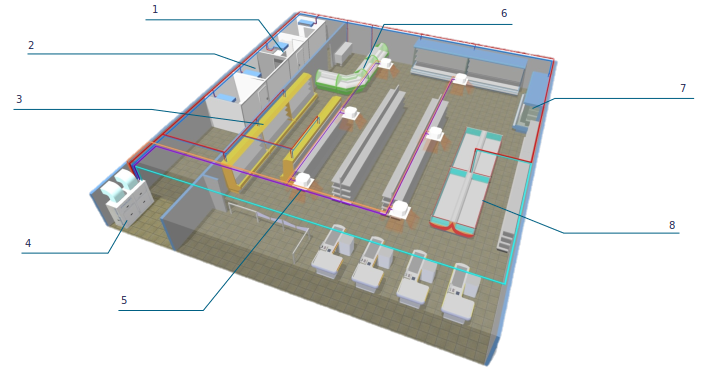
\includegraphics[width=16cm, keepaspectratio]{img/planoSupermercado}
  \caption{Plano de equipos del supermercado}
  \label{figura:planoSupermercado}
\end{figure}

\begin{enumerate}
  \item Obradores.
  \item Cámaras frigoríficas.
  \item Murales de lácteos.
  \item Central de refrigeración.
  \item Climatización\footnote[1]{En la \hyperref[figura:planoSupermercado]{Figura~\ref{figura:planoSupermercado}} aparecen unidades tipo fancoil, pero lo que en realidad hay es una serie de conductos conectados a una UTA central, que depende a su vez de una bomba de calor}.
  \item Vitrinas expositoras.
  \item Semimurales de carne, frutas y verduras.
  \item Islas de congelados.
\end{enumerate}

Kiconex emplea en sus desarrollos controladores de Dixell~\cite{marcaDixell}, en concreto los modelos \textit{IPG208} e \textit{IPG215} de \textit{iPro}~\cite{iproManual}, con los módulos de expansión IPX206 ó IPX215~\cite{iproManual}. El modelo a emplear dependerá de las especificaciones de entradas y salidas de la UTA, según especificaciones de funcionamiento del cliente. A continuación, en el \hyperref[sec:kiconex]{apartado 1 de este capítulo} se describe el software necesario para la programación de un control de este tipo.

El dispositivo inalámbrico a diseñar, mencionado en el \hyperref[chap:intro]{apartado de introducción anterior} comunicará los muebles frigoríficos: Murales de lácteos, vitrinas expositoras, semimurales e islas de congelados. El hardware empleado, descrito en el \hyperref[sec:esp32poe]{apartado 3 de este capítulo}, se basa en el chip ESP32~\cite{esp32Espressif}. Para entender el papel de este dispositivo en la red, es necesario conocer el funcionamiento de una instalación desde el punto de vista de kiconex, atendiendo a cómo se integra cada elemento. El \hyperref[sec:kiconex]{apartado 2 de este capítulo} se dedica por completo a describir la estructura de un sistema basado en kiconex.


%%%%%%%%%%%%%%%%%%%%%%%%%%%%%%%%%%%%%%%%%%%%%%%%%%%%%%%%%%%%%%%%%%%%%%%%%%%%%%%%%%%%%%%%%%%%%%%%%%%%%%
%% IPRO Y PANTALLA
%%%%%%%%%%%%%%%%%%%%%%%%%%%%%%%%%%%%%%%%%%%%%%%%%%%%%%%%%%%%%%%%%%%%%%%%%%%%%%%%%%%%%%%%%%%%%%%%%%%%%%
\break
\section{iPro y su pantalla}
\label{sec:iproypantalla}

\begin{figure}[h]
  \centering
  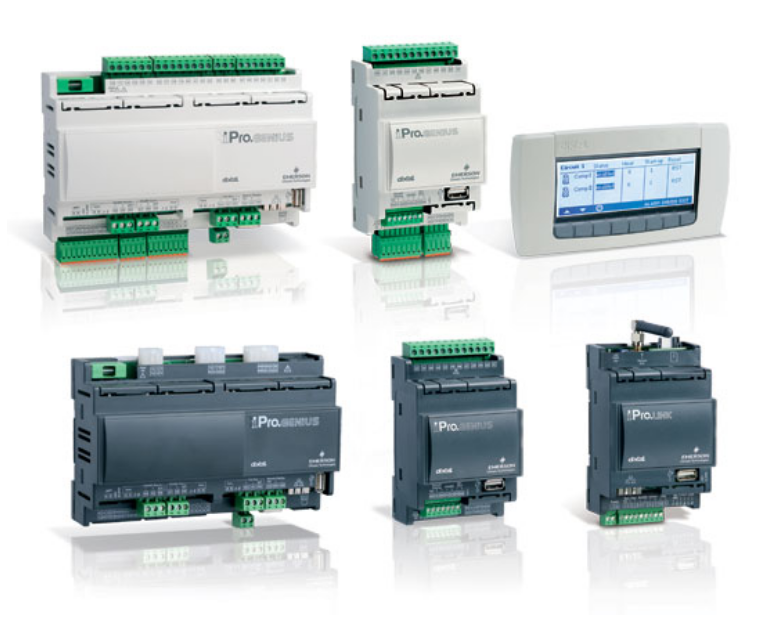
\includegraphics[width=12cm, keepaspectratio]{img/iproSeries}
  \caption{iPro Series}
  \label{figura:iproSeries}
\end{figure}

\textit{iPro} (\hyperref[figura:iproSeries]{Figura~\ref{figura:iproSeries}}) es la gama de controladores programables ofrecida por Dixell. La gama consta de controladores programables, ampliaciones de E/S, controladores para válvulas electrónicas e interfaces gráficas adaptadas para cubrir cualquier tipo de aplicación en el sector del aire acondicionado, el sector de la refrigeración y cualquier área relativa. Algunas de sus especificaciones son:

\begin{itemize}
  \item Alimentación a 24Vac/dc.
  \item Microprocesador ARM9 de 32 bits (200MHz).
  \item El programa y los parámetros se almacenan en una memoria flash permanente. No se pierden datos en caso de fallo de alimentación.
  \item Servidor web interno.
  \item Hasta 80 Mb de memoria flash, dependiendo del modelo.
  \item Entradas y salidas completamente configurables.
  \item Conexiones:
  \begin{itemize}
    \item Puerto Ethernet.
    \item Puerto USB.
    \item Conexión dedicada para un display LCD.
    \item CANBus.
    \item RS485 Master.
    \item RS485 Slave.
  \end{itemize}
\end{itemize}

Los modelos se diferencian en el tamaño (10 DIN o 4 DIN) y en el número de entradas y salidas (analógicas y digitales). La \hyperref[tab:esipro]{Tabla~\ref{tab:esipro}} recoge las especificaciones de los modelos empleados por kiconex.

\begin{table}[h]
  %\centering
  \begin{center}
    \setlength\arrayrulewidth{2pt}
    \begin{tabular}{ r | c !{\vrule width 0.25pt} c | c !{\vrule width 0.25pt} c | }
      %\Cline{2pt}{2-5}
      \hhline{*{1}{~}|*{4}{-}}
      \multirow{2}{*} & \multicolumn{2}{c|}{\cellcolor{lightgray}Controlador} & \multicolumn{2}{c|}{\cellcolor{lightgray}Módulo de Expansión}   \\ \Cline{0.25pt}{2-5}
      & \textbf{IPG208} & \textbf{IPG215} & \textbf{IPX206} & \textbf{IPX215} \\ \cline{1-1} \Cline{0.25pt}{2-5}
      \multicolumn{1}{|r|}{\textbf{Entradas analógicas}} & 6 & 10 & 7 & 10 \\
      \multicolumn{1}{|r|}{\textbf{Salidas analógicas}} & 4 & 6 & 3 & 6 \\
      \multicolumn{1}{|r|}{\textbf{Entradas digitales}} & 11 & 20 & 3 & 20 \\
      \multicolumn{1}{|r|}{\textbf{Salidas digitales (Relés)}} & 8 & 6 & 8 & 15 \\ 
      \noalign{\hrule height 2pt}
    \end{tabular}
    \caption{Especificaciones de E/S para distintos modelos de iPro.}
    \label{tab:esipro}
  \end{center}
\end{table} 

Dixell dispone de dos modelos de displays compatibles con el \textit{iPro}: \textit{VGIPG} y \textit{VTIPG}~\cite{VTIPG}. Para el diseño de dichas pantallas, se emplea el software \textit{Visoprog}~\cite{visoprog} de Dixell, que importa las variables creadas en la programación del controlador, para poder configurar en la pantalla la interacción con las mismas. 

\subsection{Programación iPro}
\label{subsec:iproprog}

Para la programación del \textit{iPro} se emplea el software \textit{ISaGRAF}~\cite{isagraf}, ya que ofrece un entorno de desarrollo estándar e internacional, soportando varios lenguajes de programación diferentes según las normas IEC61131. Se trata de un software usado en todo el mundo y que también permite simular el sistema programado. Los estándares de programación soportados son:

\begin{itemize}
  \item (\textbf{LD}) Escalera  
  \item (\textbf{FBD}) Diagrama de Bloques 
  \item (\textbf{SFC}) Tabla de Funciones Secuenciales 
  \item (\textbf{ST}) Texto Estructurado 
  \item (\textbf{IL}) Lista de Instrucciones 
  \item (\textbf{FC}) Diagrama de flujo 
\end{itemize}

Para comenzar a realizar un programa se parte de una plantilla ya preparada previamente por kiconex para configurar entradas, salidas, parámetros, alarmas, avisos, etc.. Es por ello que primero es necesario conocer las especificaciones del sistema a programar. En el código es necesario distinguir lo que es la configuración de entradas/salidas de lo que es el valor leído en las mismas.

% \begin{figure}[h]
%   \centering
%   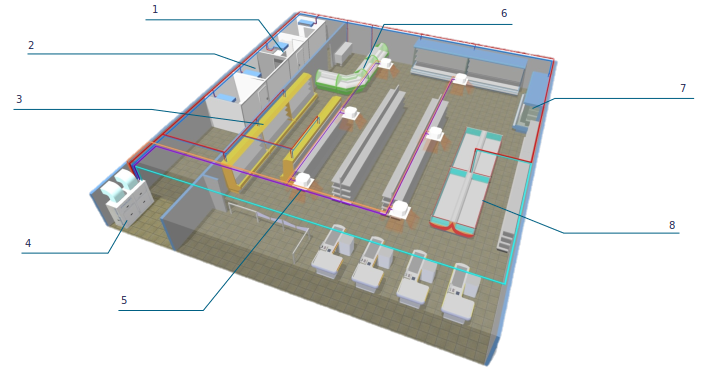
\includegraphics[width=\textwidth, keepaspectratio]{img/planoSupermercado}
%   \caption{Aspecto configuración entradas analógicas ISaGRAF}
%   \label{figura:AOisagraf}
% \end{figure}

A cada variable de parámetro, alarma, aviso, estado y entradas/salidas se le asigna una dirección de registro, como se puede ver en la \hyperref[figura:variablesIsagraf]{Figura~\ref{figura:variablesIsagraf}}. Lo habitual es destinar distintos rangos de direcciones a cada tipo de variable. 

\begin{figure}[H]
  \centering
  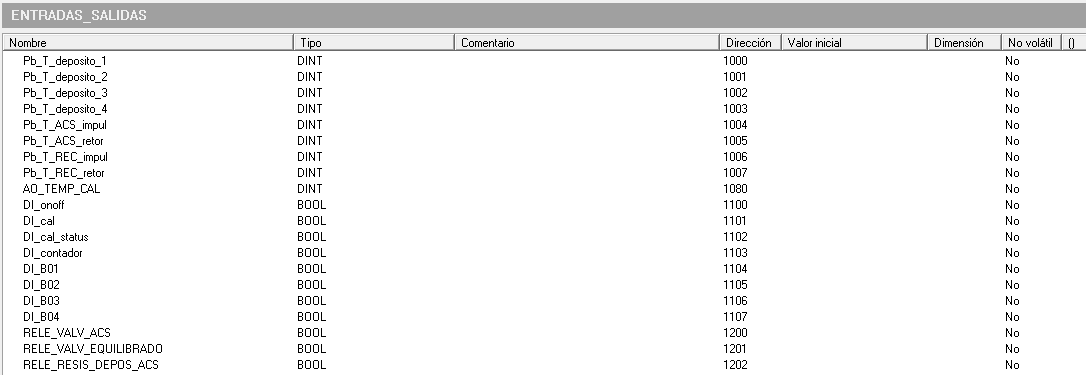
\includegraphics[width=\textwidth, keepaspectratio]{img/tablaRegistros}
  \caption{Aspecto tabla de variables en ISaGRAF}
  \label{figura:variablesIsagraf}
\end{figure}

\subsection{Configuración de la pantalla}
\label{subsec:displayconfig}

Para la configuración de la pantalla, se emplea \textit{Visoprog}, un software ofrecido por la misma marca Dixell, especialmente para su uso con los modelos \textit{VGIPG} e \textit{VTIPG}. En este caso también se ha partido de una plantilla previamente preparada por kiconex con las distintas pantallas que necesita un control como el \textit{iPro}:

\begin{figure}[H]
  \centering
  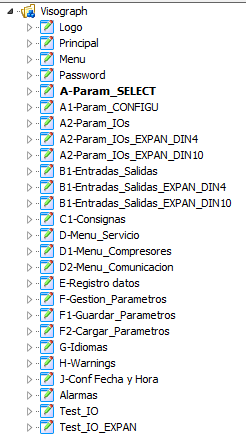
\includegraphics[width=5cm, keepaspectratio]{img/ventanasVisoprog}
  \caption{Ventanas pantalla iPro}
  \label{figura:ventanasIpro}
\end{figure}

Para usar este programa, en primer lugar se importa un fichero de registros generados por \textit{ISaGRAF}. Así es como \textit{Visoprog} los conoce y permite que el usuario interactúe con los mismos en el proceso de navegación por la pantalla, habiendo configurado previamente dicha interacción.

\textit{Visoprog} tiene también una sección destinada a textos estándar, así se puede cambiar un texto en un solo sitio, y no en los múltiples sitios en los que se está empleando. La \hyperref[figura:interfazVisoprog]{Figura~\ref{figura:interfazVisoprog}} representa el aspecto de la interfaz del programa.

\begin{figure}[H]
  \centering
  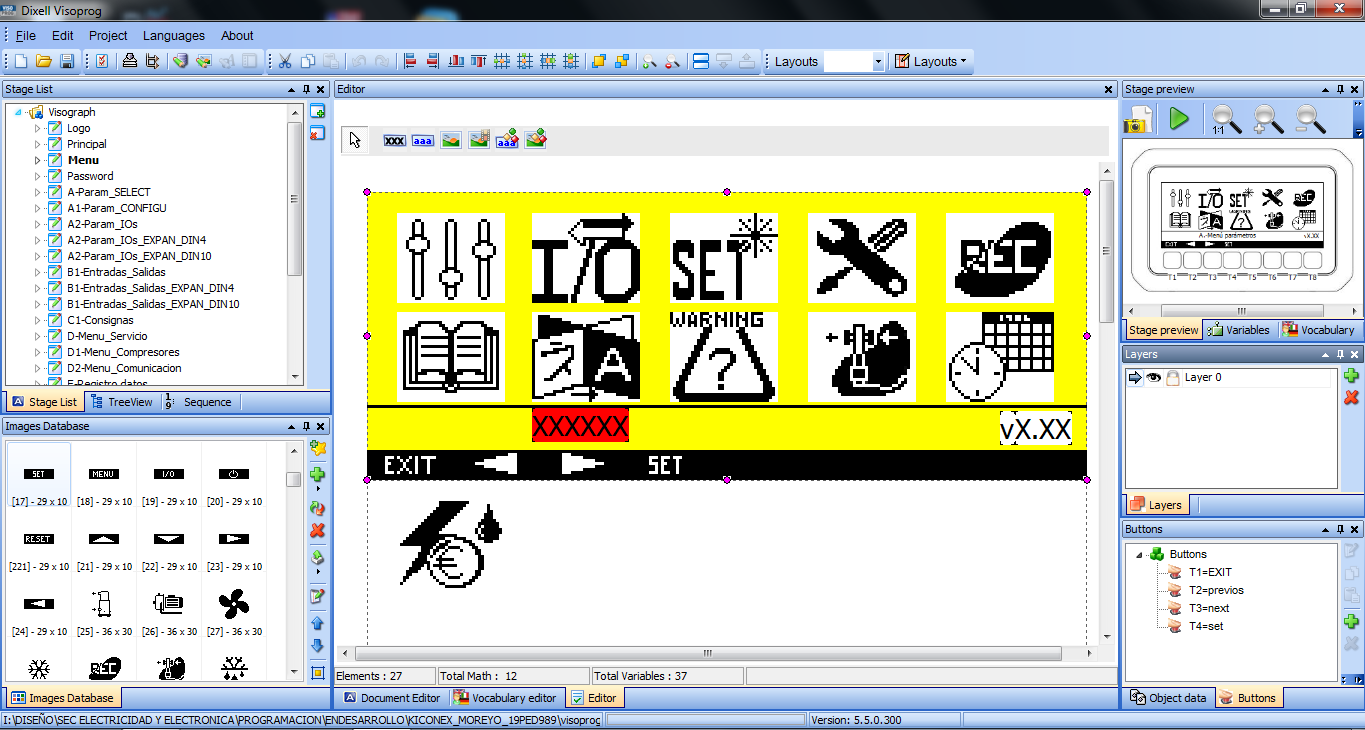
\includegraphics[width=\textwidth, keepaspectratio]{img/interfazVisoprog}
  \caption{Aspecto interfaz Visoprog}
  \label{figura:interfazVisoprog}
\end{figure}

%%%%%%%%%%%%%%%%%%%%%%%%%%%%%%%%%%%%%%%%%%%%%%%%%%%%%%%%%%%%%%%%%%%%%%%%%%%%%%%%%%%%%%%%%%%%%%%%%%%%%%
%% KICONEX
%%%%%%%%%%%%%%%%%%%%%%%%%%%%%%%%%%%%%%%%%%%%%%%%%%%%%%%%%%%%%%%%%%%%%%%%%%%%%%%%%%%%%%%%%%%%%%%%%%%%%%

\section{Kiconex}
\label{sec:kiconex}

Como ya se ha mencionado en la \hyperref[chap:intro]{introducción}, kiconex es una plataforma de supervisión y control para equipos de climatización y frío industrial. Entre sus funciones se encuentra:
\begin{itemize}
  \item \textbf{Almacenamiento en la nube} de datos de temperatura, estado de funcionamiento, presiones, etc.  
  \item \textbf{Gráficas} para visualizar la evolución de los datos en el tiempo, permitiendo compararlos. 
  \item \textbf{Control remoto}: marcha/paro, cambio de consigna, etc.
  \item \textbf{Reglas} con programaciones horarias o acciones frente a condiciones. 
  \item \textbf{Diagramas} para introducir un plano del edificio y sobre ese plano ver la temperatura de las salas y añadir botones de acción como, por ejemplo, de encendido y apagado.
  \item \textbf{Alarmas} con posibilidad de recibir alertas en caso de fallo del equipo. 
\end{itemize}

\begin{figure}[H]
  \centering
  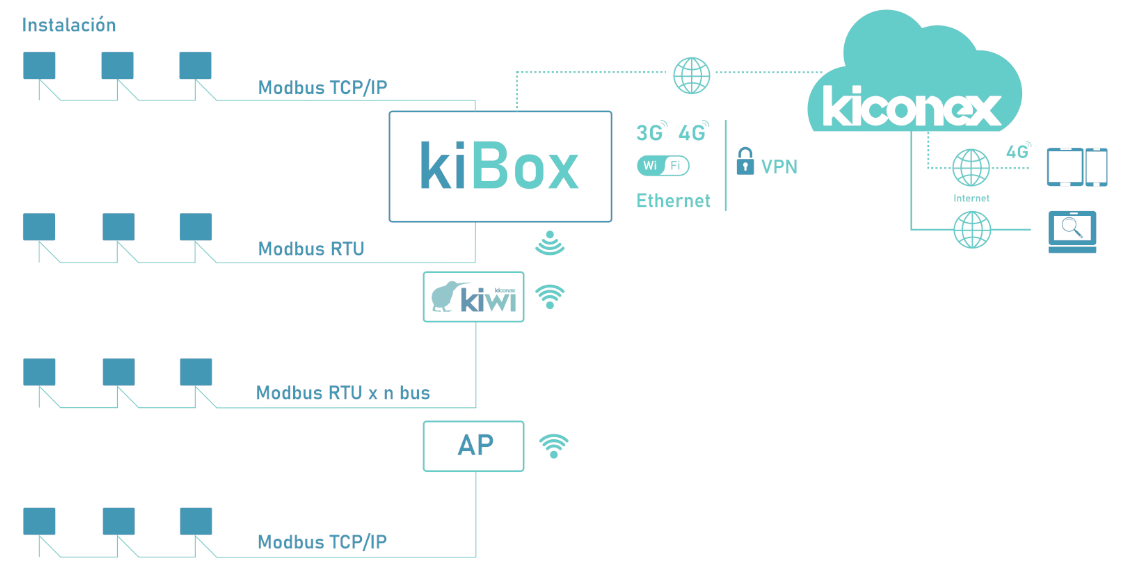
\includegraphics[width=\textwidth, keepaspectratio]{img/redKiconex}
  \caption{Red kiconex}
  \label{figura:redKiconex}
\end{figure}

Para su funcionamiento, kiconex se compone de los siguiente elementos:
\begin{enumerate}
  \item \textbf{Servidor en la nube}, donde se almacenan los datos.
  \item \textbf{Plataforma IoT para visualización y control}.  
  \item \textbf{Kibox}: hardware que actúa como pasarela entre la nube y el equipo de frío o clima. Recibe mensajes de la nube a través de MQTT, los procesa y los envía en formato Modbus al equipo final. Este último, recibe el mensaje, lo procesa y envía una respuesta que sigue el camino inverso hasta que la nube recibe la información solicitada. 
  \item \textbf{Equipos} de climatización o frío industrial: emplean el estándar industrial Modbus. La mayoría emplean Modbus RTU pero kiconex también funciona a través de Modbus TCP. Estos equipos reciben los mensajes del \textit{kibox} y le envían una respuesta.
  \item \textbf{Kiwi}: aún no está en venta, ya que se trata del dispositivo inalámbrico que se ha desarrollado en este proyecto, pero el objetivo es su actuación como esclavo Modbus, recibiendo mensajes del maestro \textit{kibox} a través de TCP-IP. \textit{Kiwi} retransmite estos mensajes actuando como maestro, a los dispositivos de frío y clima (esclavos). Es decir, \textit{kiwi} es un maestro-esclavo: maestro de cara a los equipos y esclavo de cara al \textit{kibox}.
\end{enumerate}



La plataforma de supervisión, para poder comunicarse con los controles de los equipos de frío y clima, necesita conocer sus registros. Para ello, en la plataforma existe un apartado llamado "librerías", en el cual se pueden ver y crear los mapas de registros de los controles que se necesiten. En la \hyperref[figura:libreriaPlataforma]{Figura~\ref{figura:libreriaPlataforma}} se puede ver el aspecto de una librería en la plataforma.

\begin{figure}[H]
  \centering
  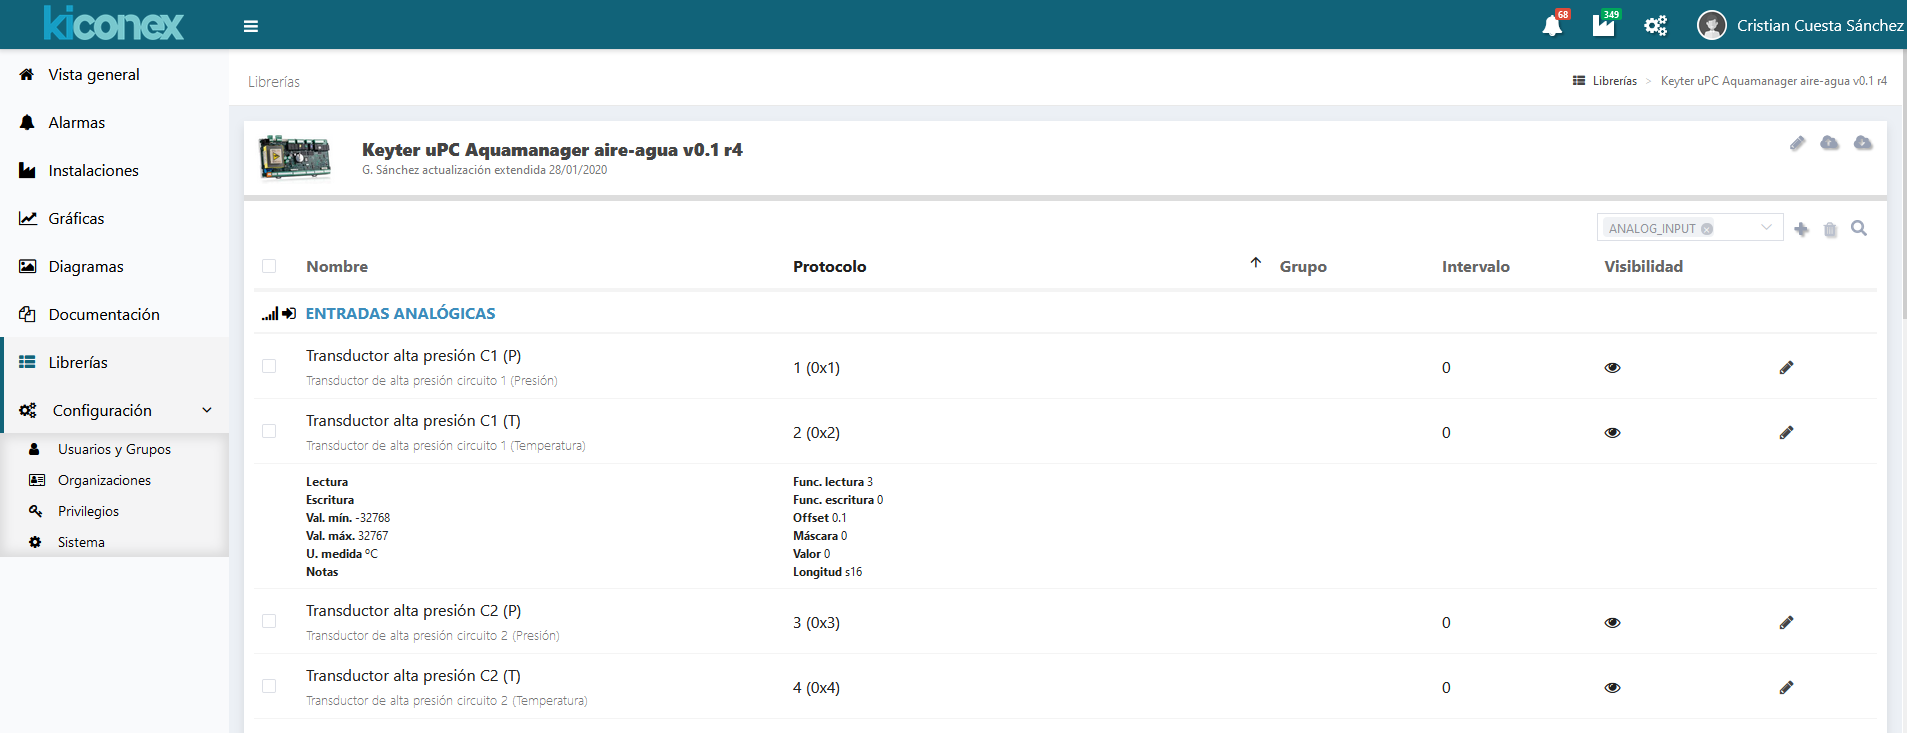
\includegraphics[width=\textwidth, keepaspectratio]{img/libreriaKiconex}
  \caption{Aspecto librería en la plataforma IoT}
  \label{figura:libreriaPlataforma}
\end{figure}

Para el caso del \textit{iPro}, en el cual el programa se diseña desde cero por kiconex, el mapeado de registros se extrae directamente del software \textit{ISaGRAF}, y se introduce en una nueva librería en la plataforma. Cuando se trata de otros controles, es el cliente quien lo consigue a través del fabricante. kiconex, gracias a su trayectoria, ya ha recopilado una gran cantidad de librerías para multitud de controles, lo que facilita mucho el proceso.

%%%%%%%%%%%%%%%%%%%%%%%%%%%%%%%%%%%%%%%%%%%%%%%%%%%%%%%%%%%%%%%%%%%%%%%%%%%%%%%%%%%%%%%%%%%%%%%%%%%%%%
%% ESP32
%%%%%%%%%%%%%%%%%%%%%%%%%%%%%%%%%%%%%%%%%%%%%%%%%%%%%%%%%%%%%%%%%%%%%%%%%%%%%%%%%%%%%%%%%%%%%%%%%%%%%%

\section{ESP32-PoE}
\label{sec:esp32poe}

\begin{figure}[H]
  \centering
  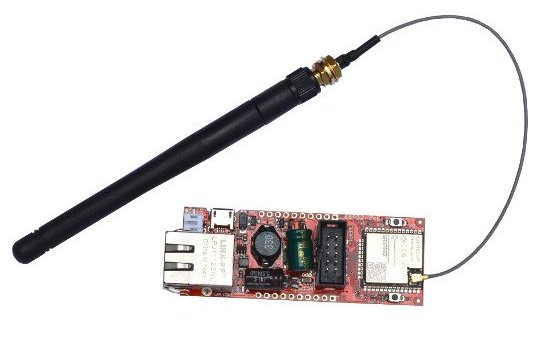
\includegraphics[width=10cm, keepaspectratio]{img/ESP32-POE}
  \caption{Olimex ESP32-PoE}
  \label{figura:imgesp32}
\end{figure}

El hardware empleado para el desarrollo del kiconex inalámbrico (\textit{kiwi}) se basa en el chip ESP32~\cite{esp32Espressif}. El modelo empleado es el Olimex ESP32-PoE (\hyperref[figura:imgesp32]{Figura~\ref{figura:imgesp32}}). Olimex~\cite{olimexEsp32product} es una empresa de Bulgaria líder en fabricación electrónica para el mercado integrado. Su modelo ESP32-PoE ha sido elegido por disponer de un puerto UEXT desde el que se puede obtener una interfaz RS-485 a través de un conversor~\cite{conversorUextProduct} (\hyperref[figura:imgconversoruext]{Figura~\ref{figura:imgconversoruext}}), para la comunicación a través de Modbus RTU. También dispone de puerto ethernet que puede usarse bien como conexión a internet vía ethernet o bien para conectar un equipo por modbus TCP. La \hyperref[figura:pinesesp32]{Figura~\ref{figura:pinesesp32}} representa los pines de entrada y salida de la placa y del conector UEXT.

\begin{figure}[H]
  \centering
  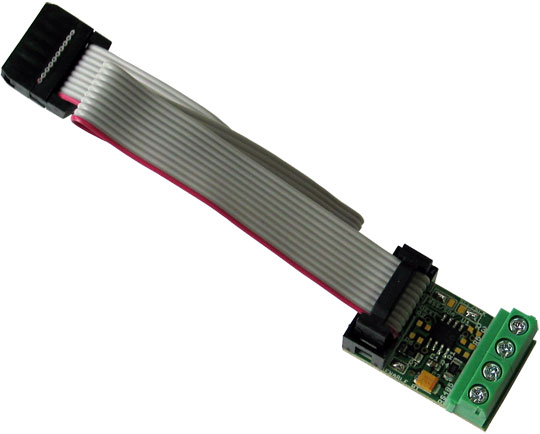
\includegraphics[width=8cm, keepaspectratio]{img/UEXT-RS485}
  \caption{Conversor UEXT-RS485}
  \label{figura:imgconversoruext}
\end{figure}

\hspace{1em}

\begin{figure}[H]
  \centering
  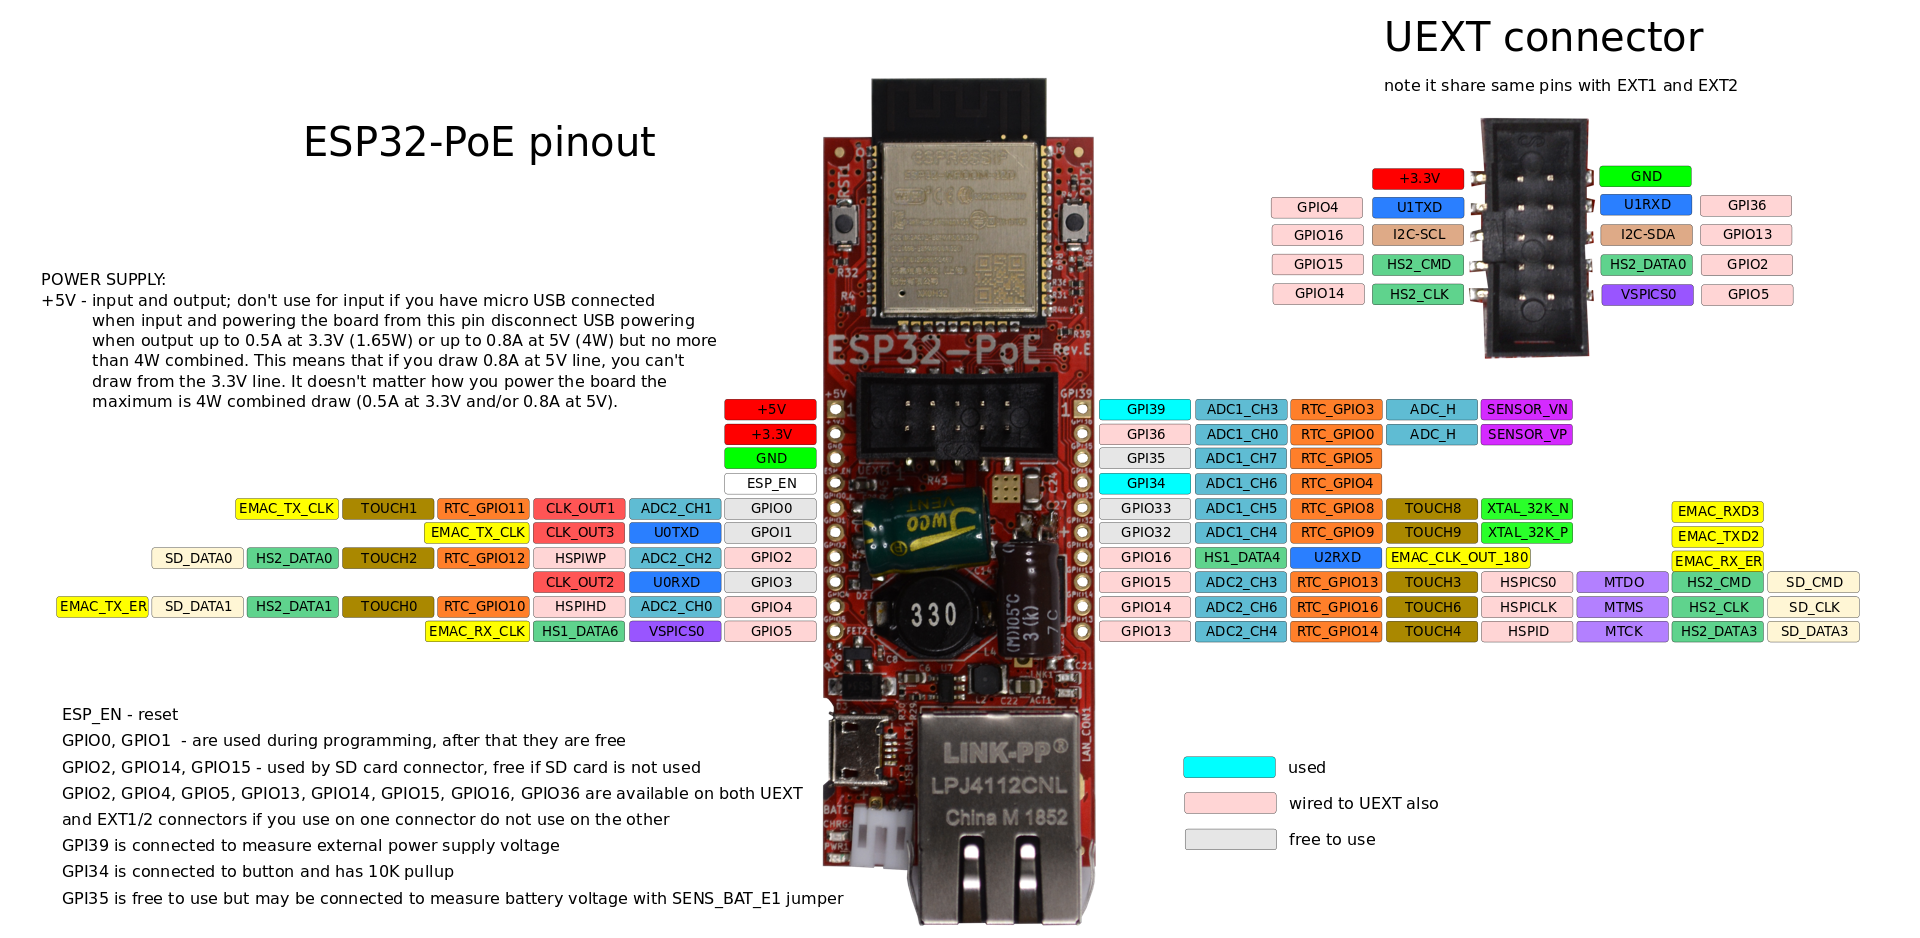
\includegraphics[width=\textwidth, keepaspectratio]{img/ESP32-POE-GPIO}
  \caption{Pines ESP32-PoE y conector UEXT}
  \label{figura:pinesesp32}
\end{figure}

Para la elaboración del código de programación del kiwi, se va a aprovechar parte del código empleado en las siguientes librerías ya existentes en github~\cite{githubWeb}:

\begin{itemize}
  \item Librería Modbus RTU, de Samuel Marco~\cite{libreriaRTUgithub}: librería necesaria para enviar mensajes vía Modbus RTU. 
  \item Librería WiFiManager, de Khoi Hoang~\cite{libreriaWiFigithub}: Servirá de punto de partida para diseñar una interfaz de configuración del \textit{kiwi}.
\end{itemize}

%\hspace{2em}

%%%%%%%%%%%%%%%%%%%%%%%%%%%%%%%%%%%%%%%%%%%%%%%%%%%%%%%%%%%%%%%%%%%%%%%%%%%%%%%%%%%%%%%%%%%%%%%%%%%%%%
%% MODBUS
%%%%%%%%%%%%%%%%%%%%%%%%%%%%%%%%%%%%%%%%%%%%%%%%%%%%%%%%%%%%%%%%%%%%%%%%%%%%%%%%%%%%%%%%%%%%%%%%%%%%%%

\section{Protocolo Modbus}
\label{sec:modbus}

Hasta este punto del documento se ha mencionado varias veces al protocolo Modbus y sus variantes: Modbus TCP y Modbus RTU, por lo que es en esta sección, y dada la importancia de este protocolo en el proyecto, donde se va a exponer de forma muy resumida sus características principales:

\begin{itemize}
  \item Distingue entre el dispositivo que solicita la información (\textbf{maestro}) y los dispositivos que proporcionan dicha información (\textbf{esclavos}). Esto significa que un esclavo no puede ofrecer información si no se le ha solicitado antes.  
  \item Para la comunicación, cada esclavo dispone de una dirección única de \textbf{8 bits}, por lo que un maestro puede tener hasta \textbf{254} esclavos.
  \item Se puede distinguir entre \textbf{Modbus TCP}, para comunicaciones vía ethernet a través de la red LAN, y \textbf{Modbus RTU}, para comunicaciones serie a través de RS232/RS485.
  \item Estructura del mensaje: el mensaje siempre se compone de: \textit{dirección del esclavo}, código de \textit{función Modbus}, \textit{dirección de registro} y \textit{cantidad de registros} a leer. En el caso del Modbus RTU, se añaden dos bytes que contienen un \textit{código CRC} para la detección de errores.
  \item Funciones: dispone de distintas funciones en función de la naturaleza de la información compartida o de los registros con los que se desea compartir información:
  \begin{itemize}
    \item \textbf{01 (0x01) Read Coils}: lee de 1 a 2000 bits de un dispositivo remoto.
    \item \textbf{02 (0x02) Read Discrete Inputs}: lee de 1 a 2000 bits de registro en un dispositivo remoto.
    \item \textbf{03 (0x03) Read Holding Registers}: lee de 1 a 125 registros de 16 bits continuos en un dispositivo remoto.
    \item \textbf{04 (0x04) Read Input Registers}: lee de 1 a 125 registros de 16 bits continuos en un dispositivo remoto.
    \item \textbf{05 (0x05) Write Single Coil}: escribe un solo bit de registro en el dispositivo remoto.
    \item \textbf{06 (0x06) Write Single Register}: escribe un solo registro de 16bits en el dispositivo remoto.
    \item \textbf{15 (0x0F) Write Multiple Coils}: escribe de 1 a 2000 bits de registro consecutivos en un dispositivo remoto.
    \item \textbf{16 (0x10) Write Multiple registers}: escribe de 1 a 123 registros 16 bits consecutivos en un dispositivo remoto.
  \end{itemize}  
\end{itemize} 

En la la web de la Modbus Organization~\cite{modbusorg} se puede encontrar la documentación que describe de forma detallada cada una de las funciones Modbus, y que información exacta contiene cada campo (byte) del mensaje.


%%%%%%%%%%%%%%%%%%%%%%%%%%%%%%%%%%%%%%%%%%%%%%%%%%%%%%%%%%%%%%%%%%%%%%%%%%%%%%%
%%%%%%%%%%%%%%%%%%%%%%%%%%%%%%%%%%%%%%%%%%%%%%%%%%%%%%%%%%%%%%%%%%%%%%%%%%%%%%%
%%%%%%%%%%%%%%%%%%%%%%%%%%%%%%%%%%%%%%%%%%%%%%%%%%%%%%%%%%%%%%%%%%%%%%%%%%%%%%%
